% @HEADER
% ***********************************************************************
% 
%            Trilinos: An Object-Oriented Solver Framework
%                 Copyright (2001) Sandia Corporation
% 
% Under terms of Contract DE-AC04-94AL85000, there is a non-exclusive
% license for use of this work by or on behalf of the U.S. Government.
% 
% This library is free software; you can redistribute it and/or modify
% it under the terms of the GNU Lesser General Public License as
% published by the Free Software Foundation; either version 2.1 of the
% License, or (at your option) any later version.
%  
% This library is distributed in the hope that it will be useful, but
% WITHOUT ANY WARRANTY; without even the implied warranty of
% MERCHANTABILITY or FITNESS FOR A PARTICULAR PURPOSE.  See the GNU
% Lesser General Public License for more details.
%  
% You should have received a copy of the GNU Lesser General Public
% License along with this library; if not, write to the Free Software
% Foundation, Inc., 59 Temple Place, Suite 330, Boston, MA 02111-1307
% USA
% Questions? Contact Michael A. Heroux (maherou@sandia.gov) 
% 
% ***********************************************************************
% @HEADER

\section{Multilevel Preconditioners with ML}
\label{chap:ml}

The ML package defines a class of preconditioners based on multilevel
methods~\cite{TuminaroTong:00a}. While technically any linear system can
be considered, ML should be used on linear systems on linear systems,
like elliptic PDEs, that are known to work well with multilevel methods.

ML is a large package, that can be used to a variety of purposes. ML
provides multilevel solvers, as well as multilevel preconditioners, and
it can handle geometric as well as algebraic methods.

In this Chapter we present:
\begin{itemize}
\item Outline the basic issues of multilevel schemes (in
  Section~\ref{ml:theoretical});
\item Present the use of ML objects as a preconditioner for an AztecOO
  solver objects (in Section~\ref{sec:ml_prec});
\item Detailes the classes ML\_Epetra::MultiLevelOperator and
  ML\_Epetra::MultiLevelPreconditioner (in
  Sections~\ref{sec:ml:operator} and \ref{sec:ml:preconditioner});
\item Outline the steps required to implement two-level domain
  decomposition methods, with a coarse grid defined using aggregation
  procedures (in Section~\ref{sec:ml_DD}).
\end{itemize}

%%%
%%%
%%%

\subsection{Theoretical Background}
\label{ml:theoretical}

Aim of this Section is to briefly present some aspects on multilevel
methods. The Section is not supposed to be exhaustive, nor complete on
this subject. The reader is referred to the existing literature for a
rigorous presentation.

\medskip

Multilevel methods require the operator to be defined on a sequence of
coarser spaces, an iterative method that evolves the solution (called a
smoother) and interpolation operators that transfer information between
the spaces. The principle behind the algorithm is that the
high-frequency errors can be efficiently solved on the fine space, while
the low-frequency are treated on the coarser one, where there
frequencies manifest themselves as high-frequencies. A very popular
multilevel methods are multigrid methods.  Geometric multigrid (GMG)
methods cannot be applied without the existence of an underlying grid
(this is their major limitation). This led to the development of
algebraic multigrid method (AMG), initiated by Ruge and St\"uben.  In
AMG, both the matrix hierarchy and the prolongation operators are
constructed just from the stiffness matrix.  Since the automatic
generation of a grid-hierarchy for GMG and especially the proper
assembly of all components would be a very difficult task for
unstructured problems, the automatic algebraic construction of a virtual
grid is a big advantage.

A function to solve (\ref{eq:linear_sys}) using a multilevel method can
be defined as follows:
\begin{verbatim}
MGM( X, B, k)
{
  if( k == 0 ) X = A_k \ B;
  else {
    X = S_k^1 (X, B);
    D = R_{k-1,k} ( B - A_k X );
    V = 0;
    MGM( V, D, k-1 );
    X = X + P_{k,k-1} V;
    X = S_k^2( U, B );
  }
}
\end{verbatim}
In the above method, $S_k^1$ and $S_k^2$ are two smoothers, $R_{k-1,k}$
is a restriction operator from level $k$ to $k-1$, and $P_{k,k-1}$ is a
prolongator from $k-1$ to $k$.

In a variational setting, the matrices $A_k$ can be constructed as
\[
A_k = R_{k-1,k} A_k P_{k,k-1}.
\]
Alternatively, when a grid is available at level $k-1$, one can
discretize the PDE operator on grid $k-1$.

\begin{remark}
  Although ML supports geometric multigrid, in this tutorial, we will
  consider multilevel methods based on aggregation schemes only.
\end{remark}

%%%
%%%
%%%

\subsection{ML as a Preconditioner for AztecOO}
\label{sec:ml_prec}

In order to use ML as a preconditioner, we need to define an
AztecOO Solver, as outlined in Chapter~\ref{chap:aztecoo}. 

ML requires the user to define a structure, to store internal data. This
structure is usually called \verb!ml_handle!:
\begin{verbatim}
ML *ml_handle;
\end{verbatim}

We intend to use ML as a ``black-box'' (or gray-box) multilevel
preconditioner, using aggregation procedures to define the multilevel
hierarchy. The variable
\begin{verbatim}
int N_levels = 10;
\end{verbatim}
defines the maximum number of levels, while
\begin{verbatim}
ML_Set_PrintLevel(3);
\end{verbatim}
toggle the output level (from 0 to 10, 10 being verbose mode and 0
silent mode).

The ML handle is created using
\begin{verbatim}
ML_Create(&ml_handle,N_levels);
\end{verbatim}
ML can accept in input very general matrices. Basically, the user has to
specify the number of local rows, and provide a function to update the
ghost nodes (that is, nodes requires in the matrix-vector product, but
assigned to another process). For Epetra matrices, this is done by the
following function
\begin{verbatim}
EpetraMatrix2MLMatrix(ml_handle, 0, &A);
\end{verbatim}
Note that \verb!A! is {\sl not} converted to ML format. Instead, proper
wrappers are defined.  (Here, \verb!A! is the Epetra matrix for which we
aim to construct a multilevel preconditioner.)

ML requires another structure, called ML\_Aggregate, to store the
information about the aggregates at various levels:
\begin{verbatim}
ML_Aggregate *agg_object;
ML_Aggregate_Create(&agg_object);
\end{verbatim}

The multilevel hierarchy is constructed with the instruction
\begin{verbatim}
N_levels = ML_Gen_MGHierarchy_UsingAggregation(ml_handle, 0,
                                               ML_INCREASING,
                                               agg_object);
\end{verbatim}
Here, \verb!0! is the index of the finest level, and the index of
coarser levels will be obtained by incrementing this value.  (We refer
to the ML manual for more details about the input parameters.)

We still need to define the smoother, for instance a symmetric Gauss-Seidel:
\begin{verbatim}
ML_Gen_Smoother_SymGaussSeidel(ml_handle, ML_ALL_LEVELS,
                               ML_BOTH, 1, ML_DEFAULT);
\end{verbatim}
and to generate the solver as
\begin{verbatim}
ML_Gen_Solver    (ml_handle, ML_MGV, 0, N_levels-1);
\end{verbatim}

Finally, we can create an Epetra\_Operator, based on the previously
defined ML hierarchy
\begin{verbatim}
ML_Epetra::MultiLevelOperator  MLop(ml_handle,comm,map,map);
\end{verbatim}
and set the preconditioning operator of our AztecOO solver,
\begin{verbatim}
solver.SetPrecOperator(&MLop);
\end{verbatim}
 
At this point, we can call \verb!Iterate()! as usual,
\begin{verbatim}
solver.Iterate(Niters, 1e-12);
\end{verbatim}

The entire code is reported in \TriExe{ml/ex1.cpp}.
The output will be approximatively as reported below.
\begin{verbatim}
[msala:ml]> mpirun -np 2 ./ex1.exe
**************************************************************
* ML Aggregation information                                 *
==============================================================
ML_Aggregate : ordering           = natural.
ML_Aggregate : min nodes/aggr     = 2
ML_Aggregate : max neigh selected = 0
ML_Aggregate : attach scheme      = MAXLINK
ML_Aggregate : coarsen scheme     = UNCOUPLED
ML_Aggregate : strong threshold   = 0.000000e+00
ML_Aggregate : P damping factor   = 1.333333e+00
ML_Aggregate : number of PDEs     = 1
ML_Aggregate : number of null vec = 1
ML_Aggregate : smoother drop tol  = 0.000000e+00
ML_Aggregate : max coarse size    = 1
ML_Aggregate : max no. of levels  = 10
**************************************************************
ML_Gen_MGHierarchy : applying coarsening
ML_Aggregate_Coarsen begins
ML_Aggregate_CoarsenUncoupled : current level = 0
ML_Aggregate_CoarsenUncoupled : current eps = 0.000000e+00
Aggregation(UVB) : Total nonzeros = 128 (Nrows=30)
Aggregation(UC) : Phase 0 - no. of bdry pts  = 0
Aggregation(UC) : Phase 1 - nodes aggregated = 28 (30)
Aggregation(UC) : Phase 1 - total aggregates = 8
Aggregation(UC_Phase2_3) : Phase 1 - nodes aggregated = 28
Aggregation(UC_Phase2_3) : Phase 1 - total aggregates = 8
Aggregation(UC_Phase2_3) : Phase 2a- additional aggregates = 0
Aggregation(UC_Phase2_3) : Phase 2 - total aggregates = 8
Aggregation(UC_Phase2_3) : Phase 2 - boundary nodes   = 0
Aggregation(UC_Phase2_3) : Phase 3 - leftovers = 0 and singletons = 0
 Aggregation time       = 1.854551e-03
Gen_Prolongator : max eigen = 1.883496e+00
ML_Gen_MGHierarchy : applying coarsening
ML_Gen_MGHierarchy : Gen_RAP
RAP time for level  0 = 5.319577e-04
ML_Gen_MGHierarchy : Gen_RAP done
ML_Gen_MGHierarchy : applying coarsening
ML_Aggregate_Coarsen begins
ML_Aggregate_CoarsenUncoupled : current level = 1
ML_Aggregate_CoarsenUncoupled : current eps = 0.000000e+00
Aggregation(UVB) : Total nonzeros = 46 (Nrows=8)
Aggregation(UC) : Phase 0 - no. of bdry pts  = 0
Aggregation(UC) : Phase 1 - nodes aggregated = 6 (8)
Aggregation(UC) : Phase 1 - total aggregates = 2
Aggregation(UC_Phase2_3) : Phase 1 - nodes aggregated = 6
Aggregation(UC_Phase2_3) : Phase 1 - total aggregates = 2
Aggregation(UC_Phase2_3) : Phase 2a- additional aggregates = 0
Aggregation(UC_Phase2_3) : Phase 2 - total aggregates = 2
Aggregation(UC_Phase2_3) : Phase 2 - boundary nodes   = 0
Aggregation(UC_Phase2_3) : Phase 3 - leftovers = 0 and singletons = 0
 Aggregation time       = 1.679042e-03
Gen_Prolongator : max eigen = 1.246751e+00
ML_Gen_MGHierarchy : applying coarsening
ML_Gen_MGHierarchy : Gen_RAP
RAP time for level  1 = 4.489557e-04
ML_Gen_MGHierarchy : Gen_RAP done
ML_Gen_MGHierarchy : applying coarsening
ML_Aggregate_Coarsen begins
Aggregation total setup time = 8.903003e-02 seconds
Smoothed Aggregation : operator complexity = 1.390625e+00.

           *******************************************************
           ***** Preconditioned CG solution
           ***** Epetra ML_Operator
           ***** No scaling
           *******************************************************

           iter:    0           residual = 1.000000e+00
           iter:    1           residual = 1.289136e-01
           iter:    2           residual = 4.710371e-03
           iter:    3           residual = 7.119470e-05
           iter:    4           residual = 1.386302e-06
           iter:    5           residual = 2.477133e-08
           iter:    6           residual = 6.141025e-10
           iter:    7           residual = 6.222216e-12
           iter:    8           residual = 1.277534e-13


           Solution time: 0.005845 (sec.)
           total iterations: 8
Residual    = 6.99704e-13
\end{verbatim}

%%%
%%%
%%%

\subsection{Class ML\_Epetra::MultiLevelOperator}
\label{sec:ml:operator}

As other Trilinos packages, ML can be compiled and run independently
from Epetra, that is, it can accept input matrix in formats different
from the Epetra\_RowMatrix or Epetra\_Operator. However, as part of the
Trilinos project, ML can be used to define a preconditioner operator for
\verb!Epetra_LinearProblem! objects (see for
instance~\cite{Epetra-Ref-Guide}). This means that, in a C++ framework,
ML can be defined as an \verb!Epetra_Operator! object, applied to an
\verb!Epetra_MultiVector!  object, and used as a preconditioner for
AztecOO.  This can be done in two ways:
\begin{itemize}
\item By defining an \verb!ML_Epetra::MultiLevelOperator! object, derived from the
  Epetra\_Operator class. The constructor of this object requires
  already filled ML\_Struct and ML\_Aggregate structures.  ML must have
  been configure with the option \newline \verb!--with-ml_epetra!.
\item By defining an \verb!ML_Epetra::MultiLevelPreconditioner! object, derived
  from the Epetra\_RowMatrix class. Basically, the constructor of
  this object demands for an Epetra\_RowMatrix  pointer and a
  Teuchos parameter list, that contains all the user's defined
  parameters. ML must have been configure with options \newline
  \verb!--with-ml_epetra --with-ml_teuchos!.
\end{itemize}

The first approach, described in Section~\ref{sec:ml:operator}, is more
general, and can be applied to geometric and algebraic multilevel
preconditioner, but it requires a deeper knowledge of the ML package.
This is because the user has to explicitly construct the ML hierarchy,
define the aggregation strategies, the smoothers, and the coarse grid
solver. The second approach, presented in
Section~\ref{sec:ml:preconditioner}, instead, although limited to algebraic
multilevel preconditioners, allows the use of ML as a black-box
preconditioner. This class automatically constructs all the components
of the preconditioner, following the parameters specified in a Teuchos
parameters' list. 

\bigskip

Class \verb!ML_Epetra::MultiLevelOperator! is defined in a header file, that must
be included as
\begin{verbatim}
#include "ml_epetra_operator.h" 
\end{verbatim}
Users may also need to include \verb!ml_config.h!,
\verb!Epetra_Operator.h!, \verb!Epetra_MultiVector.h!,
\verb!Epetra_LinearProblem.h!,  \verb!AztecOO.h!. Check the Epetra and
AztecOO documentation for more details.

Let \verb!A! be an \verb!Epetra_RowMatrix! for which we aim to construct
a preconditioner, and let \verb!ml_handle! be the structure ML requires
to store internal data, created
with the instruction
\begin{verbatim}
ML_Create(&ml_handle,N_levels);
\end{verbatim}
where \verb!N_levels! is the specified (maximum) number of levels.  As
already pointed out, ML can accept in input very general matrices.
Basically, the user has to specify the number of local rows, and provide
a function to update the ghost nodes (that is, nodes requires in the
matrix-vector product, but assigned to another process). For Epetra
matrices, this is done by the following function
\begin{verbatim}
EpetraMatrix2MLMatrix(ml_handle, 0, &A);
\end{verbatim}
and it is important to note that \verb!A! is {\sl not} converted to ML
format. Instead, \verb!EpetraMatrix2MLMatrix! defines a suitable getrow
function (and other minor data structures) that allows ML to work with
\verb!A!.

Let \verb!agg_object! a \verb!ML_Aggregate! pointer, created using
\begin{verbatim}
ML_Aggregate_Create(&agg_object);
\end{verbatim}
At this point, users have to create the multilevel hierarchy, define the
aggregation schemes, the smoothers, the coarse solver, and create the solver.
Then, we can finally create the ML\_Epetra\_Operator object
\begin{verbatim}
ML_Epetra::MultiLevelOperator  MLop(ml_handle,comm,map,map);
\end{verbatim}
(\verb!map! being the Epetra\_Map used to create the matrix) and set the
preconditioning operator of our AztecOO solver,
\begin{verbatim}
Epetra_LinearProblem Problem(A,&x,&b);
AztecOO Solver(Problem);
solver.SetPrecOperator(&MLop);
\end{verbatim}
where \verb!x! and \verb!b! are \verb!Epetra_MultiVector!'s defining
solution and right-hand side. The linear problem can now be solved as,
for instance,
\begin{verbatim}
Solver.SetAztecOption( AZ_solver, AZ_gmres );
solver.Iterate(Niters, 1e-12);
\end{verbatim}

%%%
%%%
%%%

\subsection{Class ML\_Epetra::MultiLevelPreconditioner}
\label{sec:ml:preconditioner}

Alternatively to ML\_Epetra::MultiLevelOperator, users can create
MultiLevelPreconditioner objects.  Class \verb!MultiLevelPreconditioner!
(in namespace {\tt ML\_Epetra}) is defined in a header file, that must be
included as
\begin{verbatim}
#include "ml_epetra_preconditioner.h" 
\end{verbatim}
Users may also need to include \verb!ml_config.h!,
\verb!Epetra_RowMatrix.h!, \verb!Epetra_MultiVector.h!,
\verb!Epetra_LinearProblem.h!,  \verb!AztecOO.h!. Check the Epetra and
AztecOO documentation for more details.

Table~\ref{tab:ml:aggr} reports the aggregation schemes currently
available in ML. A graphical comparison of Uncoupled and METIS is
reported in Figure~\ref{fig:ml:comparison}, for a matrix arising from
the discretization of a 2D Laplacian operator with a 9pt formula.

\begin{figure}[htbp]
  \centering
  \includegraphics[height=6cm]{ml_Uncoupled-16x16.ps} \hspace{0.5cm}
  \includegraphics[height=6cm]{ml_METIS-16x16.ps}
  \caption{Aggregates for Uncoupled (left) and METIS (right) for a 16x16 Cartesian grid.}
  \label{fig:ml:comparison}
\end{figure}

\begin{table}
\begin{center}
\begin{tabular}{ | p{5cm} | p{10cm} | }
\hline
\verb!Uncoupled! & Construct
aggregates of optimal size (for structured Cartesian grids, 3 nodes in
1D, 9 nodes in 2D, and 27 nodes 
in 3D). Works process-wise (aggregates cannot span more than 1
process). \\
\verb!MIS! & Use a maximal independent set. Aggregates can span over
processes. This scheme usually provided the best aggregates, but it is
more expensive as it requires a matrix-matrix product. \\
\verb!METIS! & Use a graph partitioning algorithm to creates the
aggregates, working process-wise. The number of nodes in each aggregate
is specified with the option {\tt aggregation: nodes per
  aggregate}. Requires ML to be configuref with {\tt
  --with-ml\_metis}. \\
\verb!ParMETIS! & As \verb!METIS!, but partition the global
graph. Requires {\tt --with-ml\_parmetis3x}. Aggregates can span
arbitrary number of processes. Global number of aggregates can be
specified with the option {\tt aggregation: global number}. \\
\hline
\end{tabular}
\caption{ML\_Epetra::MultiLevelPreconditioner: Some of the available coarsening scheme.}
\label{tab:ml:aggr}
\end{center}
\end{table}

\begin{table}
\begin{center}
\begin{tabular}{ | p{5cm} | p{10cm} | }
\hline
\verb!Jacobi! & Point-Jacobi. Damping factor is specified using
{\tt smoother: dampig factor}, and the number of sweeps with {\tt
  smoother: sweeps} \\ 
\verb!Gauss-Seidel! & Point Gauss-Seidel. \\
\verb!aztec! & Use AztecOO's built-in preconditioning functions as
smoothers. Or, use approximate solutions with AztecOO as smoothers. 
The AztecOO vectors \verb!options! and {\tt params} can be set using
{\tt smoother: aztec options} and {\tt smoother: aztec params}. \\
\hline
\end{tabular}
\caption{ML\_Epetra::MultiLevelPreconditioner: Some of the available
  smoothers.} 
\label{tab:ml:smoother}
\end{center}
\end{table}

\begin{table}
\begin{center}
\begin{tabular}{ | p{5cm} | p{10cm} | }
\hline
\verb!Jacobi! & Use Jacobi as a solver. \\
\verb!Gauss-Seidel! & Use Gauss-Seidel as a solver. \\
\verb!Amesos_KLU! & Use Amesos's KLU sequential solver. \\
\verb!Amesos_UMFPACK! & Use UMFPACK. \\
\verb!Amesos_Superludist! & Use SuperLU\_DIST. \\
\verb!Amesos_MUMPS! & Use MUMPS. \\
\hline
\end{tabular}
\caption{ML\_Epetra::MultiLevelPreconditioner: Some of the coarse matrix
  solver. Note: Amesos solvers requires 
  ML to be configured with {\tt with-ml\_amesos}, and Amesos to be
  properely configured to support the specified solver.}
\label{tab:ml:coarse}
\end{center}
\end{table}

A very simple fragment of code using this class is reported below. The
reader may refer to file
\verb!$ML_HOME/examples/ml_example_epetra_preconditioner.cpp! for a more
complex example. (In order to be effectively compiled, this example
required ML to be configured with option \verb!--with-ml_triutils!.)
\begin{verbatim}
#include "ml_include.h"
#include "ml_epetra_preconditioner.h"
#include "Teuchos_ParameterList.hpp"

...

  // A is an Epetra_RowMatrix derived class object
  // solver is an AztecOO object

  Teuchos::ParameterList MList;

  // default values for smoothed aggregation
  ML_Epetra::SetDefaults("SA",MLList);
  MLList.set("max levels",6);
  MLList.set("increasing or decreasing","decreasing");
  MLList.set("aggregation: type", "MIS");
  MLList.set("coarse: type","Amesos_KLU");
  
  ML_Epetra::MultiLevelPreconditioner * MLPrec = 
    new ML_Epetra::MultiLevelPreconditioner(A, MLList, true);

  solver.SetPrecOperator(MLPrec);
  solver.SetAztecOption(AZ_solver, AZ_gmres);
  solver.Iterate(Niters, 1e-12);

  ...

  delete MLPrec;
\end{verbatim}
The general procedure is as follows. First, the users define a Teuchos
parameters' list. Input parameters are set via method
\verb!set(ParameterName,ParameterValue)!, where \verb!ParameterName! is
a string defining the parameter, and \verb!ParameterValue! is the
specified parameter, that can be any C++ object or pointer.  This list
is passed to the constructor, together with a pointer to the matrix, and
a boolean flag.  If this flag is set to \verb!false!, the constructor
will not compute the multilevel hierarchy until when
\verb!MLPrec->ComputePreconditioner()! is called. The hierarchy can be
destroyed using \verb!MLPrec->Destroy()!.  For instance, the user may
define a code like:
\begin{verbatim}
  // A is still not filled with numerical values
  ML_Epetra::MultiLevelPreconditioner * MLPrec = 
    new ML_Epetra::MultiLevelPreconditioner(A, MLList, false);
  
  // compute the elements of A
  ...
  // now compute the preconditioner
  MLPrec->ComputePreconditioner();

  // solve the linear system, and refill A
  ...
  // destroy the previously define preconditioner, and build a new one
  MLPrec->Destroy();
  MLPrec->ComputePreconditioner();
\end{verbatim}
In this fragment of code, the user defines the ML preconditioner, but
does not create the preconditioner in the construction phase. This is of
particular interest, for example, when ML is used in conjuction with
nonlinear solvers (like NOX~\cite{NOX-home-page}).

We point out that the input parameter list is {\sl copied} in the
construction phase, hence later changes to \verb!MLList! will not affect
the preconditioner. Should one need to modify parameters in the
\verb!MLPrec!'s internally stored parameter list, he can proceed as
follows:
\begin{verbatim}
  ParameterList & List = MLPrec->GetList();
\end{verbatim}
and then directly modify \verb!List!.

\medskip

All ML options can have a common prefix, specified by the
user in the construction phase. For example, suppose that we require
\verb!ML: ! to be the prefix. The constructor will be
\begin{verbatim}
  MLLIst.set("ML: aggregation: type", "METIS");
  ML_Epetra::MultiLevelPreconditioner * MLPrec = 
    new ML_Epetra::MultiLevelPreconditioner(*A, MLList, true, Prefix);
\end{verbatim}
where \verb!Prefix! is a char array containing \verb!ML: !.

Note that spaces are important: Do not include leading or trailing
spaces, and separate words by just one space! Mispelled parameters will
not be used, and can be detected calling method \verb!PrintUnused()!
{\sl after} the construction of the multilevel hierarchy. 

For a detailed list of all the parameters, we refer to the ML user's
guide.  Here, we report the most used parameters in
Tables~\ref{tab:ml:aggr}, \ref{tab:ml:smoother} and \ref{tab:ml:coarse}.


%%%
%%%
%%%


\subsection{Two-Level Domain Decomposition Preconditioners with ML}
\label{sec:ml_DD}

In order to use the example reported in this Section, one should compile
ML with the configure flag \verb!--with-ml_metis!. In this way, ML will
use the graph decomposition library METIS to create the coarse-level
matrix\footnote{Note that ML has to be aware of the location of the
  METIS include files and the METIS library. The user can use the
  configure flags {\tt --with-incdirs} and {\tt --with-ldflags}.  Please
  type {\tt configure --help} in the ML subdirectory for more
  information. If you don't have METIS, or you don't want to
  re-configure ML, you will be able to run the example of this Section.
  However, you will be limited to use only one aggregate per process.}.

Two-level domain decomposition methods have been proved to be very
effective for the iterative solution of many different kind of linear
systems.  For some classes of problems, a very convenient way to define
the coarse grid operator is to use aggregation procedure. This is very
close to what presented in Section~\ref{sec:ml_prec}. The main
difference is that only two level methods are considered, and that the
coarse grid remains of (relatively) small size. The idea is to define a
small number of aggregates on each process, using a graph decomposition
algorithm (as implemented in the library METIS, for
instance)\footnote{Aggregation schemes based on ParMETIS as also
  available. Please refer to the help of the ML {\tt configure} for more
  details.}. This can be done as follows.

The linear system matrix \verb!A!, here coded as an Epetra\_CrsMatrix,
corresponds to the discretization of a 2D Laplacian on a Cartesian
grid. \verb!x! and \verb!b! are the solution vector and the right-hand
side, respectively.

The AztecOO linear problem is defined as
\begin{verbatim}
  Epetra_LinearProblem problem(&A, &x, &b);
  AztecOO solver(problem);
\end{verbatim}

At this point, we can create the Teuchos parameters' list, with the
following parameters:
\begin{verbatim}
  ParameterList MLList;

  ML_Epetra::SetDefatuls(("DD",MLList);

  MLList.set("max levels",2);
  MLList.set("increasing or decreasing","increasing");

  MLList.set("aggregation: type", "METIS");
  MLList.set("aggregation: nodes per aggregate", 16);
  MLList.set("smoother: pre or post", "both");
  MLList.set("coarse: type","Amesos_KLU");
  MLList.set("smoother: type", "aztec");
\end{verbatim}
The last option tells ML to use the Aztec preconditioning function as a
smoother. Aztec requires an integer vector \verb!options! and a double
vector \verb!params!. Those can be defined as follows:
\begin{verbatim}
  int options[AZ_OPTIONS_SIZE];
  double params[AZ_PARAMS_SIZE];
  AZ_defaults(options,params);
  options[AZ_precond] = AZ_dom_decomp;
  options[AZ_subdomain_solve] = AZ_icc;
  MLList.set("smoother: aztec options", options);
  MLList.set("smoother: aztec params", params);
\end{verbatim}
Note that {\sl all} Aztec preconditioners can be used as smoothers for
ML. 
At this point we can create the ML preconditioner as
\begin{verbatim}
  ML_Epetra::MultiLevelPreconditioner * MLPrec =
    new ML_Epetra::MultiLevelPreconditioner(A, MLList, true);
\end{verbatim}
and check that no options have been mispelled, using
\begin{verbatim}
  MLPrec->PrintUnused();
\end{verbatim}
AztecOO solver is called using
\begin{verbatim}
  solver.SetPrecOperator(MLPrec);

  solver.SetAztecOption(AZ_solver, AZ_cg_condnum);

  int Niters = 500;
  solver.SetAztecOption(AZ_kspace, 160);

  solver.Iterate(Niters, 1e-12);
\end{verbatim}
Finally, some (limited) information about the preconditioning phase are
obtained using
\begin{verbatim}
  cout << MLPrec->GetOutputList();
\end{verbatim}

The entire code is reported in \TriExe{ml/ex2.cpp}.

%%%
%%%
%%%

\subsection{Concluding Remarks on ML}
\label{sec:ml_concluding}

More documentation about ML can be found in
\cite{ML-home-page,TuminaroTong:00}.

